\chapter{Introduction}
\label{ch:cryo-intro}

\section{LBNF Cryogenics Infrastructure}
\label{sec:cryo-intro-fd}

The scope of the LBNF Cryogenics Infrastructure includes the design, 
procurement, fabrication, testing, delivery and installation
oversight of the following components:
\begin{itemize}
 \item {Four identical cryostats to contain the liquid argon (LAr) 
       and the single-phase (or dual-phase) time projection chambers (TPCs)} 
 \item {A comprehensive cryogenic system that meets the performance 
       requirements for}
 \begin{itemize} 
  \item {purging, cooling down and filling the cryostats}
  \item {acquiring and maintaining the LAr temperature within 
        $\pm$1 K range around nominal temperature (88.3 K)} 
  \item {purifying the LAr via constant filtration using recirculation pumps
         outside the cryostats}
 \end{itemize}
\end{itemize}

The reference design for the LBNF cryogenics infrastructure 
encompasses the following components:

\begin{itemize}
\item Four identical 10-metric-kiloton (fiducial mass) membrane cryostats 
\item Receiving facilities for LAr and LN$_2$ tanker trucks 
\item Transfer system to deliver argon gas for liquefaction and 
      nitrogen gas for refrigeration system from the
      surface to the underground cavern area
\item A closed loop LN$_2$ refrigeration system for condensing GAr
\item Boil-off gas reliquefaction equipment
\item LAr-purification facilities
\item Cryostat-purge facilities
\end{itemize}


The conceptual reference design for the DUNE far detector (FD) specifies four  
rectangular cold vessels each measuring 15.1~m internal width, 14.0~m internal 
height and 62.0~m internal length - each vessel contains a total mass of 
approximately 17~kt of LAr and between 3 and 5\% of Ar gas operating at a 
pressure of 75 mbarg, depending on the final TPC design. The 
membrane design is commonly 
used for liquefied natural gas (LNG) storage and transport 
tanker ships (Figure~\ref{fig:memb-tank-int}) and has been 
proven to be a viable option for LArTPC experiments. 
A membrane tank 
is made of a stainless-steel liner to contain the liquid cryogen. 
The pressure loading of the liquid cryogen is transmitted 
through rigid foam insulation to the surrounding structural support 
which provides external support for the liner. The membrane 
liner is corrugated to provide strain relief resulting from 
temperature-related expansion and contraction (Figure~\ref{fig:prim-barrier}).


\begin{cdrfigure}[Interior of a LNG tanker ship]{memb-tank-int}{Interior of a LNG tanker ship. 
The tank shown is 24~m high by 35~m wide with interior grid-like 
corrugations on a 0.34~m pitch. By comparison, a single LBNF 
cryostat is 14.0~m high by 15.1~m wide.}
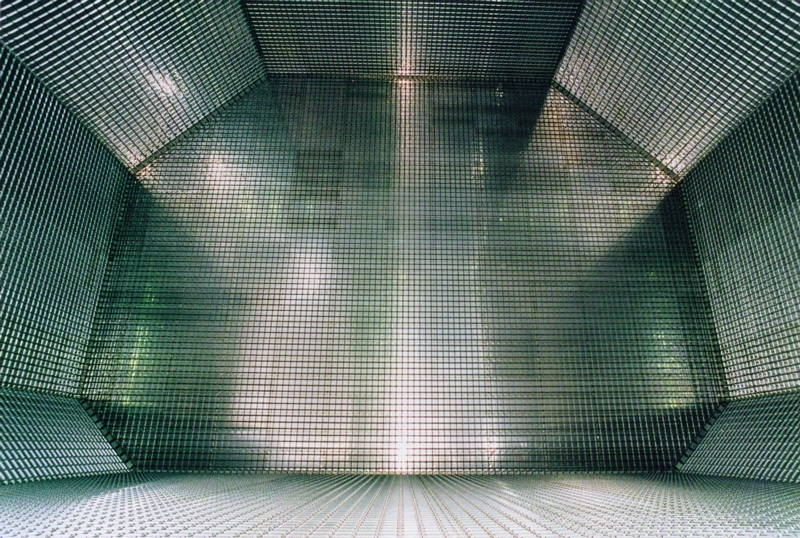
\includegraphics[width=.8\textwidth]{v5ch2-memb-tank-int}
\end{cdrfigure}

\begin{cdrfigure}[Primary membrane section]{prim-barrier}{Primary membrane section (courtesy GTT)}
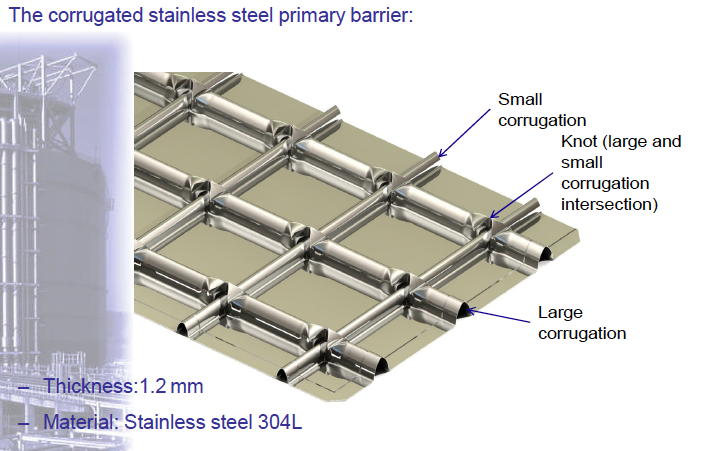
\includegraphics[width=.8\textwidth]{v5ch2-prim-barrier}
\end{cdrfigure}


The advantages offered by the membrane design relative to a self-supporting cryostat are:
\begin{itemize}
\item Efficient use of the underground cavern volume due to its positioning 
close to the rock on floor and sides, which reduces the civil construction 
costs for the project
\item Higher ratio of usable (fiducial) mass to active (total) mass
\end{itemize}

Two membrane cryostat vendors have been 
identified. Those vendors are GTT (Gaztransport \& Technigaz) and 
IHI (Ishikawajima-Harima Heavy Industries). Each is technically capable 
of delivering a membrane cryostat that meets the design requirements for 
the LBNF. To provide clarity, only one vendor is represented here (GST 
system from GTT); this is for informational purposes only and should not 
be construed as preferring GTT over IHI. Nothing inherent in the IHI 
design changes the design approach. 


\section{Design Parameters}
\label{sec:cryo-cryosys-params}

The requirements and parameters for the cryostat and cryogenics system 
design are within the LBNF requirement documentation~\cite{lar-fd-req}~\cite{lar-fd-req-traceback}  
and the parameter tables~\cite{lar-fd-params} and~\cite{cryo-params}, respectively. The 
overarching system requirements are to provide a high-purity, 
stable liquid argon environment for the TPC and to provide 
mechanical support for the TPC. For components that pass 
through the ullage (the vapor space above the LAr), no 
sources of reliquefaction may be present. Tables 
\ref{tab:param-summ-LBNF} and \ref{tab:cryo-reqs} 
offer a brief overview of parameters for a single 
cryostat of LBNF.

\begin{cdrtable}[Design parameters for one LBNF Cryostat]{l p{8cm} }{param-summ-LBNF}{Design parameters for one LBNF Cryostat}
Parameter &  Value \\ \toprowrule
Cryostat Internal Volume &  13,107 m$^3$ \\ \colhline
Total LAr Mass & 17.2 kt \\ \colhline
Cryostat Inside Depth & 14.0 m \\ \colhline
Cryostat Inside Width & 15.1 m \\ \colhline
Cryostat Inside Length & 62.0 m  \\ \colhline
Cryostat Outside Height & 18.116 m \\ \colhline
Cryostat Outside Width & 19.216 m \\ \colhline
Cryostat Outside Length & 66.116 m \\ \colhline
Insulation &  Reinforced Polyurethane of 90~cm thickness; \\
           &  two (inner/outer) layers around secondary \\
           &  containment (30/60~cm per each layer) \\ \colhline
Primary Membrane (GTT Design) & 1.2 mm thick type 304L stainless steel \\
                              & with corrugations on 340 mm $\times$ 503 mm \\
                       & rectangular pitch\\ \colhline
Secondary Containment (GTT Design) & $\approx$ 0.07 mm thick aluminum between \\ 
                            & fiberglass cloth; overall thickness is \\
                            & 0.8 mm located between insulation layers \\ \colhline
External Vapor Barrier Thickness & 10 mm \\
(Steel Plates)                   &       \\ \colhline
External Support Structure Thickness & 1.148 m (Steel) \\
On Sides & \\ \colhline
External Support Structure Thickness & 1.148 m (Steel) \\
Top and Bottom & \\ \colhline
LAr Temperature & 88.3 $\pm$ 1 K \\ \colhline
Minimum LAr Depth (Liquid Head) & 13.2 m \\ \colhline
Ullage Operating Pressure & 130 mbarg (range: 50$-$200 mbarg) \\ \colhline
Pressure at Bottom & 1,948 mbarg \\ \colhline
Cryostat Design Pressure & 350 mbarg \\
\end{cdrtable}


\begin{cdrtable}[Summary of parameters for membrane cryostat at the 4850L]{ p{0.43\textwidth} p{0.5\textwidth}}{cryo-reqs}{Summary of parameters for membrane cryostat at the 4850L (the bottom of the Ross shaft)}
Property & Reference-Design Cryostat\\ \toprowrule
Personnel Access to Cavern & Ross shaft\\ \colhline
Equipment Transport to Cavern & Ross shaft (main transport), Yates shaft \\ \colhline
Construction Access to Pit & From above highbay \\ \colhline
Type of Crane in Cavern & Mobile construction \\ \colhline
Base & Steel structure \\ \colhline
Side Walls & Steel structure \\ \colhline
Heating System & Redundant/replaceable electric system \\ \colhline
Roof & Steel structure \\ \colhline
Vapor Barrier & Steel plates  \\ \colhline
Insulation/Secondary Barrier/Membrane & GST system by GTT \\ \colhline
TPC & Individual 2.3 m $\times$ 6.0 m frames lowered through \\
    & a dedicated roof opening. Assembled within \\
    & cryostat and suspended by hangers passing \\
    & through the roof. \\ \colhline
LAr Containment System & Stainless Steel Primary Membrane; \\
                       & Secondary Barrier \\
\end{cdrtable}


%%%%%%%%%%%%%%%%%%%%%%%%%%%%%%%%%%%%%%%%%%%%%%%%%%%%%%%%%%%%%%%%%%%%%%



\nomenclature{ADC}{analog-to-digital converter}
\nomenclature{APA}{anode plane assembly}
\nomenclature{APD}{avalanche photodiodes}
\nomenclature{ArgoNeuT}{Mini LArTPC Exposure to Fermilab's NuMI Beam}
\nomenclature{ASIC}{application-specific integrated circuit}
\nomenclature{BGR}{band-gap reference}
\nomenclature{CAD}{computer-aided design}  
\nomenclature{CDF}{one of two decommissioned collider detectors at Fermilab's Tevatron, along with D-Zero}  
\nomenclature{CF}{conventional facilities} 
\nomenclature{CFD}{computerized fluid dynamics} 
\nomenclature{CPA}{cathode plane assembly}
\nomenclature{DAQ}{data acquisition}
\nomenclature{DCM}{data concentrator module}
\nomenclature{DC}{direct current}
\nomenclature{DCM}{Data concentrator modules}
\nomenclature{D-Zero}{one of two decommissioned collider detectors at Fermilab's Tevatron, along with CDF}
\nomenclature{EM}{electromagnetic}
\nomenclature{ENC}{equivalent noise charge}
\nomenclature{ESH}{Environment, Safety and Health}
\nomenclature{FEM}{front-end module}
\nomenclature{FESHM}{Fermilab's ES\&H Manual}
\nomenclature{FFT}{Fast Fourier Transform}
\nomenclature{FIRUS}{Fire and Utilities; Fermilab site-wide, high-reliability, remote monitoring system used to monitor building fire panels and various utilities throughout the lab}
\nomenclature{FLARE}{Fermilab Liquid Argon Experiments}
\nomenclature{FPGA}{field-programmable gate array}
\nomenclature{FR-4}{flame resistant 4}
\nomenclature{FSE}{field-shaping electrode}
\nomenclature{GAr}{gaseous argon}
\nomenclature{GLACIER}{NASA's General Laboratory Active Cryogenic International Space Station Experiment Refrigerator}
\nomenclature{LNGS}{Gran Sasso National Laboratory}
\nomenclature{G10/FR4}{a fire rated electrical-grade dielectric made with and epoxy material reinforced with a woven fiberglass mat}
\nomenclature{GTT}{Gaztransport \& Technigaz}
\nomenclature{HSSD}{High Sensitivity Smoke Detection}
\nomenclature{HV}{high voltage}
\nomenclature{HVAC}{heating, ventilation and air conditioning}
\nomenclature{ICARUS}{Imaging Cosmic and Rare Underground Signals, experiment at the LNGS}
\nomenclature{INFN}{Istituto Nazionale della Fiscia Nucleare} 
\nomenclature{IHI}{Ishikawajima-Harima Heavy Industries}
\nomenclature{IT}{integration prototype}
\nomenclature{IU}{Indiana University}
\nomenclature{LANNDD}{Liquid Argon Neutrino and Nucleon Decay Detector}
\nomenclature{LAPD}{Liquid Argon Purity Demonstrator}
\nomenclature{LAr}{liquid argon}
\nomenclature{LAr1}{one-kiloton LAr prototype for LBNE's LAr-FD}
\nomenclature{LAr-FD}{LBNE's Liquid Argon Far Detector}
\nomenclature{LArSoft}{a reconstruction software package for LAr detectors}
\nomenclature{LArTPC}{liquid argon time projection chamber}
 \nomenclature{LBNE}{Long-Baseline Neutrino Experiment}
\nomenclature{LED}{light-emitting diode}
\nomenclature{LEM}{large electron multiplier}
\nomenclature{LEMO}{a push-pull connector made by the LEMO company in Switzerland}
\nomenclature{LHe}{liquid helium}
\nomenclature{LN}{liquid nitrogen, also written LN$_2$ and LN2}
\nomenclature{LNG}{liquefied natural gas}
\nomenclature{LOTO}{lockout/tagout; an OSHA safety practice }
\nomenclature{LPG}{liquefied petroleum gas}
\nomenclature{LVDS}{low-voltage differential signaling}
\nomenclature{MCT}{membrane cryostat test}
\nomenclature{MicroBooNE}{A 100-ton LArTPC located along Fermilab's Booster neutrino beamline }
\nomenclature{MINERvA}{A neutrino-scattering experiment that uses the NuMI beamline at Fermilab}
\nomenclature{MINOS}{Main Injector Neutrino Oscillation Search, a Fermilab experiment}
\nomenclature{MIP}{minimum ionizing particle}
\nomenclature{MIT}{Massachusetts Institute of Technology}
\nomenclature{MOS}{metal-oxide semiconductor}
\nomenclature{MOSFET}{metal-oxide-semiconductor field-effect transistor}
\nomenclature{MTU}{master timing unit}
\nomenclature{MUX}{multiplex}
\nomenclature{Bis-MSB}{1,4-bis[2-(2-methylphenyl)ethenyl]-benzene, a wavelength-shifting chemical}
\nomenclature{MTS}{Materials Test Stand}
\nomenclature{N or N2}{nitrogen}
\nomenclature{NASA}{National Aeronautics and Space Administration}
\nomenclature{NBTI}{negative bias temperature instability}
\nomenclature{NC}{neutral current}
\nomenclature{NICADD}{Northern Illinois Center for Accelerator and Detector Development NOvA}
\nomenclature{NIM}{Nuclear Instruments and Methods (journal)}
\nomenclature{NIST}{National Institute of Standards and Technology}
\nomenclature{NIST}{National Institute of Standards and Technology}
\nomenclature{NSF}{National Science Foundation}
\nomenclature{NOvA}{NuMI Off-Axis Neutrino Appearance experiment at Fermilab}
\nomenclature{OD}{outer diameter}
\nomenclature{ODH}{oxygen deficiency hazard}
\nomenclature{OPERA}{Oscillation Project with Emulsion-Racking Apparatus, at CERN and LNGS}
\nomenclature{OSHA}{Occupational Safety and Health Administration}
\nomenclature{PC}{personal computer}
\nomenclature{PC-4}{Fermilab building, Proton Center building number 4}
\nomenclature{PCI}{peripheral component interconnect}
\nomenclature{PDA}{photon detection assembly}
\nomenclature{PDE}{photon-detection efficiency}
\nomenclature{PE}{photo-electron}
\nomenclature{PLC}{programmable logic controller}
\nomenclature{PMT}{photomultiplier tube}
\nomenclature{PPE}{personnel protective equipment}
\nomenclature{PRV}{pressure-relief valve}
\nomenclature{QC}{quality control}
\nomenclature{RC}{resistive capacitive}
\nomenclature{ROOT}{An object oriented framework for large-scale data analysis developed at CERN}
\nomenclature{SCR}{silicon controlled rectifier}
\nomenclature{SDSTA}{South Dakota Science and Technology Authority}
\nomenclature{SIMOPS}{simultaneous operations study}
\nomenclature{SiPM}{Silicon photomultiplier}
\nomenclature{SM}{stress-migration}
\nomenclature{S/N}{signal-to-noise }
\nomenclature{SS}{stainless steel}
\nomenclature{TC}{thermal cycling}
\nomenclature{TDDB}{time-dependent dielectric breakdown}
\nomenclature{TDU}{timing distribution unit}
\nomenclature{TPB}{tetraphenyl butadiene, a wavelength shifting chemical}
\nomenclature{TPC}{Time Projection Chamber}
\nomenclature{USB}{universal serial bus}
\nomenclature{UV}{ultraviolet}
\nomenclature{VME}{a computer bus standard}
\nomenclature{VUV}{vacuum ultraviolet light}
\nomenclature{WARP}{Wimp Argon Program}
\nomenclature{WBS}{Work Breakdown Structure}
\nomenclature{WLS}{wavelength shifter}

\nomenclature{A}{ampere (also mA, kA)   }
\nomenclature{atm}{atmosphere}
\nomenclature{bar}{bar (also mbar, etc.)}
\nomenclature{barg}{bar gauge (deprecated per Wikipedia)}
\nomenclature{b}{barn, a measure of cross section; bit (also Mb, Gb, etc.)}
\nomenclature{B}{byte (also MB, GB, etc.)}
\nomenclature{Bq}{becquerel}
\nomenclature{C}{coulomb}
\nomenclature{cf}{cubic foot (also ft$^3$)}
\nomenclature{cfm}{cubic feet per meter (also ft$^3$/m)}
\nomenclature{Ci}{curie}
\nomenclature{eV}{electron-volt (also keV, MeV, GeV) }
\nomenclature{F}{farad (also pF, nF )}
\nomenclature{ft}{foot or feet }
\nomenclature{gal}{gallon}
\nomenclature{gpm}{gallons per minute (also gal/min)} 
\nomenclature{G}{gauss (also mG) or gradient (in magnets)}
\nomenclature{g}{gram (also mg, kg)}
\nomenclature{Hz}{hertz (s-1)}
\nomenclature{h}{hour}
\nomenclature{in}{inch }
\nomenclature{K}{kelvin} 
\nomenclature{l}{liter}
\nomenclature{m}{meter (also nm, micron, mm, cm, km) }
\nomenclature{min}{minute }
\nomenclature{MICA}{type of dielectric material used in capacitors}
\nomenclature{MS}{mega samples}
\nomenclature{N}{newton}
\nomenclature{NPO}{type of dielectric material used in capacitors}
\nomenclature{QFP}{quad flat pack}
\nomenclature{R}{roentgen}
\nomenclature{Pa}{pascal}
\nomenclature{psi}{pounds per square inch}
\nomenclature{rad}{radian (also mrad) }
\nomenclature{s}{second (also ns, $\mu$s, ms) }
\nomenclature{scfm}{standard cubic foot per minute }
\nomenclature{SHV}{safe high voltage, a type of HV cable connector}
\nomenclature{t}{ton}
\nomenclature{T}{Tesla}
\nomenclature{V}{volt (also mV, kV, MV)}
\nomenclature{VA}{volt-ampere (also mVA, kVA, MVA)}
\nomenclature{VAC}{Volts alternating current (also mVAC, kVAC)}
\nomenclature{VUV}{vacuum ultraviolet}
\nomenclature{W}{watt (also mW, kW, MW) }
\nomenclature{yd}{yard }
